\documentclass[border=10pt]{standalone}

\usepackage{tikz}
\usepackage{tikzsymbols}
\usetikzlibrary{calc,patterns,shapes.geometric}

\def\centerarc[#1](#2)(#3:#4:#5){\draw[#1] ($(#2)+({#5*cos(#3)},{#5*sin(#3)})$) arc (#3:#4:#5);}

\begin{document}
	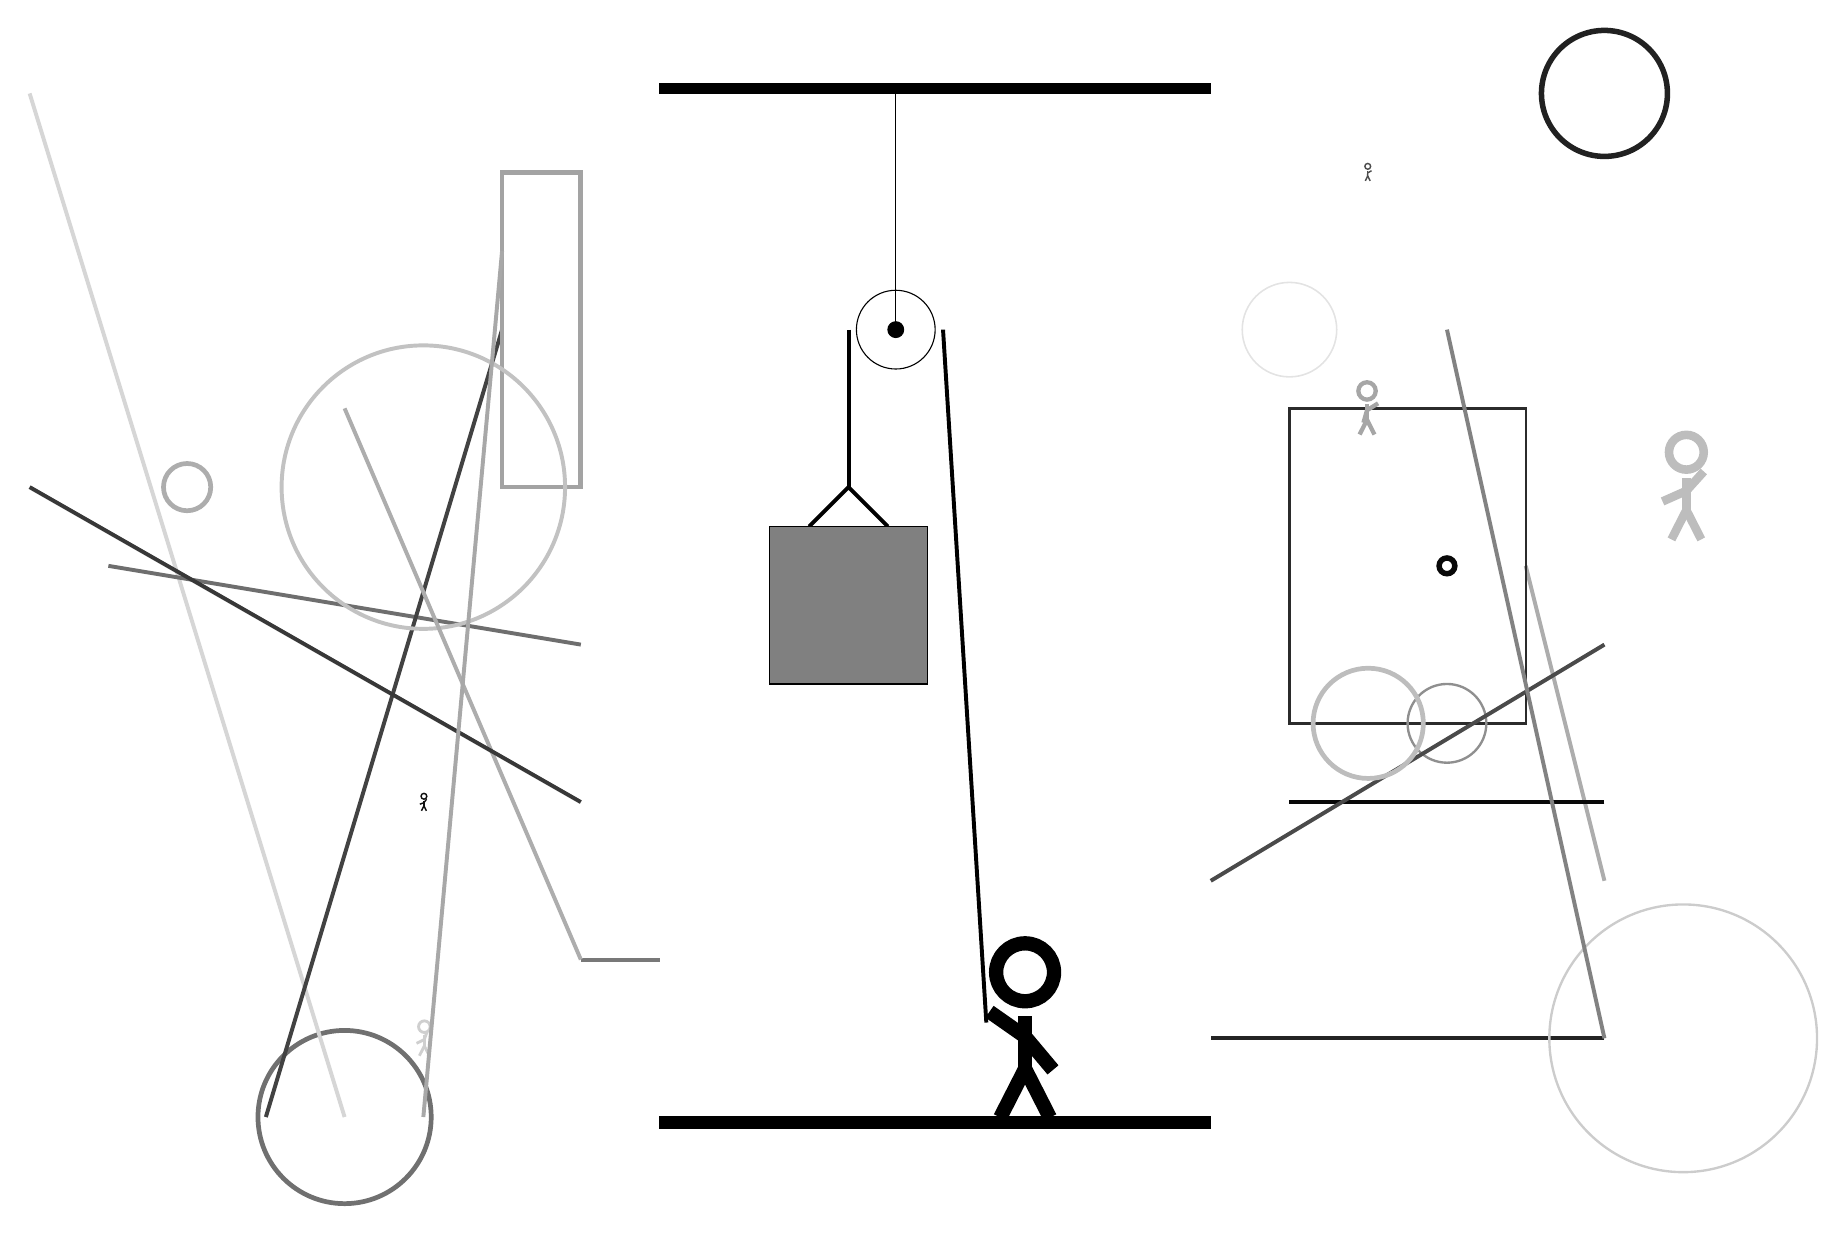
\begin{tikzpicture}
		%%%%% START %%%%%
		
		\draw[fill=black] (-2, 10) rectangle (5, 10.125);
		
		\draw (1, 7) circle (0.5);
		\draw[fill=black] (1, 7) circle (0.1);
		\draw (1, 10) -- (1, 7);
		
		\draw[line width=0.5mm] (-0.1, 4.5) -- (0.4, 5.0) -- (0.9, 4.5);
		\draw[fill=black!50] (-0.6, 4.5) rectangle (1.4, 2.5);
		
		\draw[line width=0.5mm] (0.4, 7) -- (0.4, 5.0);
		\centerarc[line width=0.5mm](1, 7)(0:180:0.6);
		\draw[line width=0.5mm](1.6, 7) -- (2.15, -1.8);
		
		\node at (2.6, -1.9) {\Strichmaxerl[10][-35][-50]};
		
		\draw[line width=0.5mm, color=black!32](10, 0) -- (9, 4);
		
		\draw [line width=0.6mm, color=black!56](-6, -3) circle (1.1);
		\draw [line width=0.7mm, color=black!97](8, 4) circle (0.1);
		\draw [line width=0.2mm, color=black!11](6, 7) circle (0.6);
		\draw[line width=0.5mm, color=black!16](-6, -3) -- (-10, 10);
		
		\draw[line width=0.5mm, color=black!97](10, 1) -- (6, 1);
		
		\draw[line width=0.5mm, color=black!53](-2, -1) -- (-3, -1);
		\draw[line width=0.3mm, color=black!83] (6, 2) rectangle (9, 6);
		\draw[line width=0.5mm, color=black!57](-3, 3) -- (-9, 4);
		\draw[line width=0.5mm, color=black!86](10, -2) -- (5, -2);
		
		\draw[line width=0.5mm, color=black!74](-4, 7) -- (-7, -3);
		\draw [line width=0.7mm, color=black!87](10, 10) circle (0.8);
		\draw[line width=0.6mm, color=black!36] (-3, 9) rectangle (-4, 5);
		
		\node[line width=0.7mm, color=black!19] at (-5, -2) {\Strichmaxerl[2][26][71]};
		\node[line width=0.7mm, color=black!26] at (11, 5) {\Strichmaxerl[6][24][48]};
		\node[line width=0.3mm, color=black!94] at (-5, 1) {\Strichmaxerl[1][20][53]};
		
		\node[line width=0.2mm, color=black!35] at (7, 6) {\Strichmaxerl[3][74][32]};
		\node[line width=0.4mm, color=black!70] at (7, 9) {\Strichmaxerl[1][87][28]};
		\draw [line width=0.5mm, color=black!24](-5, 5) circle (1.8);
		
		\draw [line width=0.3mm, color=black!44](8, 2) circle (0.5);
		\draw [line width=0.3mm, color=black!20](11, -2) circle (1.7);
		
		\draw[line width=0.5mm, color=black!71](5, 0) -- (10, 3);
		\draw[line width=0.5mm, color=black!32](-6, 6) -- (-3, -1);
		\draw[line width=0.5mm, color=black!49](8, 7) -- (10, -2);
		\draw [line width=0.6mm, color=black!32](-8, 5) circle (0.3);
		
		\draw [line width=0.6mm, color=black!26](7, 2) circle (0.7);
		\draw[line width=0.5mm, color=black!81](-4, 0) -- (-4, 0);
		\draw[line width=0.5mm, color=black!78](-3, 1) -- (-10, 5);
		
		\draw[line width=0.5mm, color=black!34](-4, 8) -- (-5, -3);
		
		\draw[fill=black] (-2, -3) rectangle (5, -3.15);
		
		%%%%% END %%%%%
	\end{tikzpicture}
\end{document}